% !TEX root = BA-Bericht.tex
\chapter{Stand der Technik}\label{ch:StandDerTechnik}
% Auch "Stand der Forschung" oder "Stand der Praxis"

% Bezogen auf die eigenen Zielsetzungen und Fragestellungen soll aufgezeigt werden, wie andere
% dieses oder ähnliche Probleme gelöst haben. Worauf können Sie aufbauen, was müssen Sie neu
% angehen? Wodurch unterscheidet sich Ihre Lösung von anderen Lösungen? Für wissenschaftlich
% orientierte Arbeiten sei hier explizit auf (Balzert, S. 66 ff) verwiesen.

Dieses Kapitel zeigt den aufgrund der Zielsetzung und Fragestellung ermittelten Stand der Technik auf.
Dies beinhaltet die Resultate der Recherche, sowie einen Beschrieb der Technologien auf welchen diese Arbeit aufbaut.
Im ersten Abschnitt~\fullref{sec:techintro} wird ein Einstieg in das Thema Anonymisierungsnetzwerke geboten, wobei die Begrifflichkeiten Privatsphäre und Anonymität erklärt sowie grundsätzliche Einschränkungen von Anonymisierungsnetzwerken erläutert werden.
Im zweiten Abschnitt~\fullref{sec:technischeKonzepte} wird genauer auf die Technologie von I2P eingegangen.
Darin wird die Funktionsweise von I2P genauer erläutert und relevante technische Konzepte erklärt.

\section{Einführung in die Technologie}\label{sec:techintro}
% TODO Wichtige technologischen Grundlagen / Wissenswertes

Da sich diese Arbeit um ein Anonymisierungsnetzwerk dreht und somit die Privatsphäre der Benutzer gewährleistet werden soll (siehe Abschnitt~\fullref{sec:ziel}),
werden zunächst diese Begrifflichkeiten erklärt.
Anschliessend werden grundsätzliche Beschränkungen von Anonymisierungsnetzwerken aufgezeigt.
Schlussendlich wird genauer auf I2P selber eingegangen, da es sich hier um die Netzwerkschicht von DIVA.EXCHANGE handelt.

\subsection{Privatsphäre und Anonymität}\label{sec:privacy_anonymity}

Im DIVA.EXCHANGE-Netzwerk sollen digitale Güter austauscht werden können.
Dies ohne sich gegenseitig zu kennen und ohne sich gegenseitig vertrauen zu müssen.
Das heisst in Folge, dass die Anonymität und Privatsphäre der Benutzer gewährleistet werden müssen.
Anonymität und Privatsphäre sind jedoch nicht dasselbe.
Im Weiteren werden diese beiden Begriffe differenziert und verglichen.
Diese Thematik wurde schon in einer vorherigen Arbeit (siehe \cite[S. 9]{maric_untersuchung_2020}) mit DIVA.EXCHANGE behandelt,
wobei bereits eine Definition von Privatsphäre und Anonymität erarbeitet wurde.

Komplette Anonymität ist dann erreicht, wenn nicht auf die wahre Identität eines Benutzers geschlossen werden kann,
das heisst, es fehlen jegliche Identitätsmerkmale, die einen Hinweis auf die reale Person geben würden.
Anonymität ist jedoch auch ein Spektrum.
Ein Internetbenutzer kann zum Beispiel teilweise anonym sein, indem er ein Pseudonym wie einen Benutzername verwendet.
Dabei handelt es sich bei einem Benutzernamen auch um ein Identitätsmerkmal.
Wenn dieses Pseudonym jedoch mit Identitätsmerkmalen der richtigen echten Person in Zusammenhang gebracht wird,
ist die Anonymität wiederum verloren. \parencite[S. 8-9]{maric_untersuchung_2020}

Mit Hilfe von Anonymität kann auch die Privatsphäre geschützt werden.
Anonymität ist jedoch nicht zwingend notwendig, um die Privatsphäre der Benutzer oder den Datenschutz zu gewährleisten.
Privatsphäre kann zum Beispiel nur schon durch Verwendung von Verschlüsselung erreicht werden.
Auch kann die Anonymität sogar verloren gehen, versucht man die Privatsphäre zu schützen,
dies zum Beispiel wenn Verschlüsselung mit einer Signatur verwendet wird, die auf die wahre Identität eines Benutzers zurückschliessen lässt.
Anonymität kann durch Verschlüsselung, sowie auch durch Weiterleiten oder Durchmischen von Nachrichten erreicht werden.

\subsection{Anonymisierungsnetzwerke}

Es gibt eine Vielzahl von verschiedenen Anonymisierungsnetzwerken.
Wobei \glstext{tor} (\glsname{tor}) wahrscheinlich das Bekannteste und meistgenutzte ist.
In einer vorherigen Arbeit wurde I2P mit TOR verglichen und es wurde festgestellt, dass I2P die Voraussetzungen für Privatsphäre und Anonymität des Software-Prototypen von DIVA.EXCHANGE \parencite[S.~28-30]{maric_untersuchung_2020} erfüllt.
Deshalb wird I2P nun als Grundstein für das Netzwerklayer von DIVA.EXCHANGE eingesetzt.
Somit wird in dieser Arbeit lediglich das Anonymisierungsnetzwerk \glsname{i2p} behandelt und nicht weiter auf andere Anonymisierungsnetzwerke eingegangen.

\subsection{Das Anonymitätstrilemma}\label{sec:anonymitytrilemma}

Beim Design eines anonymen Kommunikationsprotokolls gibt es grundsätzliche Einschränkungen, die zu beachten sind.
Es gilt die folgenden drei Aspekte abzuwägen und einen Kompromiss zwischen diesen zu finden:

\begin{itemize}
    \item Der Anonymitätsgrad von Sender und Empfänger einer Nachricht.
    \item Die zur Kommunikation benötigte Netzwerkbandbreite.
    \item Die Latenzzeiten und Verzögerungen der zu übermittelnden Nachrichten.
\end{itemize}

Dabei ist es nicht möglich ein Protokoll zu designen, welches einen hohen Anonymitätsgrad bietet, wenig Netzwerkbandbreite benötigt und tiefe Latenzzeiten vorweist. \parencite[S.~1]{das_anonymity_2018}
Höhere Anonymität geht also immer auf Kosten von höherer Latenzzeiten oder mehr benötigter Netzwerkbandbreite, oder auf Kosten von beidem.
(siehe auch Abbildung~\fullref{fig:anonimitytrilemma}).

\begin{figure}[H]
    \centering
    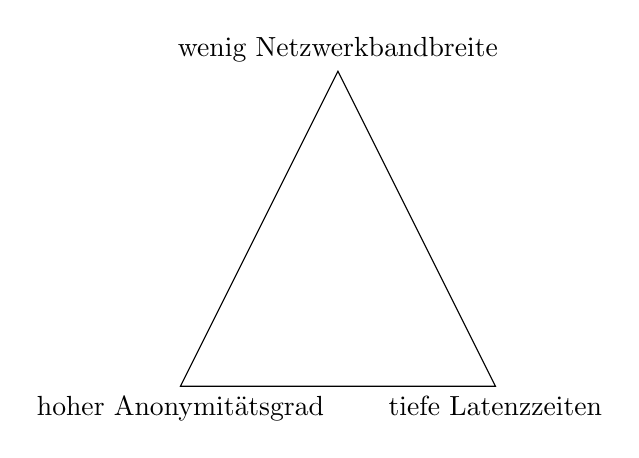
\begin{tikzpicture}
      \draw (0,0) node[anchor=north]{hoher Anonymitätsgrad}
        -- (4,0) node[anchor=north]{tiefe Latenzzeiten}
        -- (2,4) node[anchor=south]{wenig Netzwerkbandbreite}
        -- cycle;
    \end{tikzpicture}
    \caption{Das Anonymitätstrilemma}\label{fig:anonimitytrilemma}
\end{figure}

Ein Anonymisierungsnetzwerk könnte beispielsweise auf Kosten der Netzwerkbandbreite implementiert werden, indem die Nachrichten jeweils an alle Netzwerkteilnehmer versendet werden.
Somit könnte mindestens der Empfänger verschleiert werden.
Auch gibt es die Möglichkeit, mehr Anonymität zu schaffen, indem der Netzwerkverkehr ergänzt wird
oder vermischt wird mit anderem Netzwerkverkehr.

Umgekehrt könnte ein Anonymisierungsnetzwerk auf Kosten der Latenz implementiert werden.
Werden Nachrichten über mehrere Netzwerkknoten geleitet, könnte man Empfänger und Sender verschleiern.
Jedoch hätte dies höhere Latenzzeiten zur Folge,
da dieselbe Nachricht mehrmals nacheinander von verschiedenen Netzwerkknoten bearbeitet werden müsste.
Zusätzlich könnte bei diesem Ansatz ein Netzwerkknoten extra ein Netzwerkpaket zwischenspeichern und zeitverzögert weiterschicken.
Dies würde das Anonymisierungsnetzwerk noch besser gegen timing-basierte Deanonymisierungsangriffe und Korrelation von Netzwerkverkehr schützen.
Und schliesslich gibt es Netzwerke bei welchen Anonymität keine Rolle spielt, wie beispielsweise beim üblichen ``User Datagram Protocol'' (UDP).
Es ist dann möglich hohe Bandbreite sowie niedrige Latenzzeiten zu erreichen.

Es gilt abzuwägen, welche der Aspekte für das zu designende Protokoll wichtig sind.
Es muss entschieden werden, wo man ein Schwerpunkt setzt und welche Aspekte man somit auch vernachlässigt, um einen guten Kompromiss zu finden. \parencites[S.~1-2]{das_anonymity_2018}

\subsection{The Invisible Internet Protocol (\glsname{i2p}) }

Kurz gesagt ist ``\glstext{i2p}'' (\glsname{i2p}) ein dezentrales Mischnetzwerk, in dem verschlüsselte Nachrichten ausgetauscht werden können.
Es handelt sich hier um ein eigenständiges Overlay-Netzwerk, welches auf den darunterliegenden Protokollen UDP und TCP aufbaut.
Mit einem Mischnetzwerk ist gemeint, dass Nachrichten durch Knoten des Netzwerks weitergeleitet werden, um den Sender und den Empfänger einer Nachricht zu verschleiern. Dieser Mischvorgang wird bei I2P Garlic-Routing genannt (siehe Abschnitt \fullref{sec:garlic_routing}).
Auch gilt es zu unterstreichen, dass \textit{Nachrichten} ausgetauscht werden.
I2P ist \textit{nachrichtenbasiert} und verhält sich in diesem Sinne ähnlich wie UDP \parencite[S.~1]{zantout_i2p_2011}.
Es gibt dementsprechend keine Garantien, dass, wenn eine Nachricht versendet wird, die Daten in der richtigen Reihenfolge, komplett oder überhaupt ankommen.
Es gibt jedoch Erweiterungen auf dem Netzwerk, welche diese Garantien (ähnlich, wie es sie bei TCP gibt) wieder herstellen können.
Zudem bietet I2P eine Ende-zu-Ende-Verschlüsselung von Nachrichten.
Die Nachrichten sind also vom Sender bis zum Empfänger verschlüsselt.

Während das TOR-Netzwerk ursprünglich entwickelt wurde, um auf das öffentliche Internet via Outproxies zuzugreifen,
liegt bei I2P der Fokus darin anonym auf Dienste, die innerhalb des Netzwerks angeboten werden, zuzugreifen.
Jedoch besteht bei TOR ebenfalls die Möglichkeit, netzwerkinterne Dienste anzubieten mittels ``TOR Hidden Services''. Umgekehrt gibt es aber auch bei I2P die Möglichkeit, mit Hilfe von Outproxies, auf das normale Internet zuzugreifen \parencite[S. 2]{ehlert_i2p_2011}.
Dienste, die innerhalb des Netzwerks angeboten werden, sind zum Beispiel Bit-Torrent für File-Sharing, Webseiten (sogenannte ``eepsites''), oder auch Chat-Dienste wie IRC (Internet Relay Chat).\\
\parencite[p.~3-4]{de_boer_invisible_2019,noauthor_i2p_nodate}


\section{Technische Konzepte von I2P}
\label{sec:technischeKonzepte}
% TODO Konzepte in diesem Feld welche für den Leser relevant sind

In diesem Abschnitt werden wichtige Begrifflichkeiten und technische Konzepte im Bezug auf I2P genauer erklärt und unter die Lupe genommen.

\subsection{I2P-Router}\label{sec:router}

Ein I2P-Router ist ein einzelner Teilnehmer, ein Knoten oder auch ein Peer im I2P-Netzwerk.
Ein Router kann Nachrichten weiterleiten und somit im Netzwerk mischen, aber auch empfangen, oder versenden.
Es gibt zwei verschiedene Implementationen von I2P-Router-Software, welche auch zusammenarbeiten können und gemeinsam ein Netzwerk bilden können.
Die ursprüngliche Implementation des I2P-Routers, welche auch I2P genannt wird, wurde in Java programmiert.
In dieser Arbeit wird jedoch lediglich die später entwickelte und schlankere C++-Implementation auch genannt ``i2pd''\footnote{Webseite: \url{https://i2pd.website/}} (Invisible Internet Protocol Daemon), untersucht.

\subsection{Destinations}

Ein I2P-Router kann eine beliebige Anzahl an Destinations (Zielorten) im I2P-Netzwerk zur Verfügung stellen.
Eine Destination hat immer mindestens eine Adresse, mit welcher andere Netzwerkteilnehmer einen netzwerkinternen Service erreichen können.
Wurde eine Destination mit einem Service definiert, erstellt der I2P-Router beim Aufstarten ein Schlüsselpaar.
Dieses wird für die Verschlüsselte Kommunikation mit dem Service benötigt.
Zudem wird aus dem Public-Key immer auch eine netzwerkinterne Adresse für den Service abgeleitet.
Diese Adresse nennt sich eine b32-Addresse.
Dies ist eine 52-Zeichen-lange aus Kleinbuchstaben und Zahlen bestehender Name.
Zudem hat diese die Endung \lstinline|.b32.i2p| damit klar ist, dass dieser Name innerhalb des Overlay-Netzwerks aufgelöst werden muss.
Eine b32-Adresse sieht also zum Beispiel so aus:\\
\lstinline|b2cdodoyqg5v6go56bkaevvw777e2wyiflqh6zyyyxugy4cqlzuq.b32.i2p|.
\parencite{noauthor_naming_nodate}

\subsection{Tunnels}

Wenn man im Bereich vom Netzwerken über Tunneling redet, geht es immer darum ein Kommunikationsprotokoll in ein anderes einzubetten. \parencite{noauthor_duden_nodate}
Die gesamte Menge an Tunnels und I2P-Routern bildet somit ein Overlay-Netzwerk.
Bei I2P ist ein Tunnel ein \textit{unidirektionaler} Kommunikationsweg durch eine ausgewählte Liste an I2P-Routern.
Die Tunnels werden aus Anonymitätsgründen alle zehn Minuten zerstört und wieder neuaufgebaut.
Ähnlich wie beim Onion-Routing wird hier die Nachricht mehrfach verschlüsselt, damit die Zwischenknoten nicht in die Nachricht hineinsehen können, jedoch trotzdem die benötigen Routing-Informationen haben, um diese an den richtigen Ort weiterzuleiten.
Es wird also eine Verschlüsselungsschicht nach der anderen bei jedem Hop durch das Netzwerk abgebaut,
ähnlich wie man die verschiedenen Schichten einer Zwiebel abnehmen kann.

Bei I2P gibt es verschiedene Arten von Tunnels, welche in den folgenden Abschnitten genauer differenziert werden.
\parencites{noauthor_intro_nodate}[S.~2]{liu_empirical_2014}

\subsubsection{Inbound- und Outbound-Tunnels}
Da die Tunnels ein unidirektionalen Kommunikationsweg bieten, gibt es Inbound- und Outbound-Tunnels,
wobei die Inbound-Tunnels zum Empfang und die Outbound-Tunnels zum Versand von Nachrichten dienen.
Inbound-Tunnels sind also Nachrichteneingänge und Outbound-Tunnels sind Nachrichtenausgänge.
Jeder I2P-Router kann eine beliebige Anzahl Inbound- und Outbound Tunnels erstellen.
Dies hat zur Folge, dass wenn eine Nachricht beantwortet wird, die Antwort nicht über den gleichen Weg wieder zurückkommt.
\parencite{noauthor_intro_nodate}

\subsubsection{Exploratory--Tunnels}

Exploratory-Tunnels sind Tunnels mit tiefer Bandbreite und werden dazu verwendet, um Tunnels aufzubauen, zu verwalten, oder zu zerstören.
Sie werden also nicht für sensible Operationen bezüglich Privatsphäre eingesetzt.
Genauer gesagt wird mit Hilfe dieser Tunnels das I2P-Netzwerk nach weiteren I2P-Routern durchforscht, um weitere Netzwerkteilnehmer zu finden, und die NetDb (siehe \fullref{sec:netdb}) heruntergeladen.
\parencite[S.~4]{conrad_survey_2014}

\subsubsection{Client-Tunnels}

Client-Tunnels sind Tunnels mit grösserer Kapazität und Bandbreite. Um solche gute Tunnels zu finden und zu erstellen werden erst die Exploratory-Tunnels benötigt, welche andere I2P-Router erforschen (siehe Abschnitt~\fullref{sec:tunnelerstellung}).
Sie werden einerseits zum Abfragen der LeaseSets aus der NetDb eingesetzt (siehe Abschnitt~\fullref{sec:netdb}).
Andererseits sind dies auch die Tunnels, welche die Nachrichten von Applikationen und Services, die im I2P-Netzwerk angeboten werden übermitteln.
\parencites[S.~4]{conrad_survey_2014}{noauthor_tunnelimplementierung_nodate}

\subsubsection{Länge der Tunnels}

Jedes Tunnel hat eine Länge, welche von jedem I2P-Knoten selber festgelegt werden kann.
Die Tunnellänge gibt an, durch wie viele Knoten eine Nachricht, die durch das Tunnel verschickt wird, geroutet wird.
Für jeden Hop im Tunnel wird die Nachricht in eine zusätzliche Verschlüsselungsschicht eingehüllt,
sodass wissen die Router jeweils nur Bescheid wissen, von welchem anderen Router sie eine Nachricht erhalten haben und an welchen Router die Nachricht weitergeleitet werden soll.
Ein Router mitten im Tunnel weiss also schlussendlich nie, von wem und an wen eine Nachricht verschickt wurde.
Die Länge eines Tunnels kann auch 0 betragen.
In diesem Fall wird eine Nachricht die durch das Tunnel verschickt wird, durch keine weitere Knoten geroutet.
Hierbei kann jeder Knoten selber festlegen, wie lange seine eigenen Tunnels sind.
Je länger ein Tunnel ist, desto mehr Anonymität bietet er.
Jedoch geht dies auf Kosten der Latenz aufgrund der zusätzlichen Hops.
Die Standardlänge von Exploratory-Tunnels beträgt 2, alle anderen Tunnels haben eine Standardlänge von 3.
Da der Ausgang oder das Ende eines Outbound-Tunnels eines I2P-Routers mit einem Eingang oder Anfang eines Inbound-Tunnels verbunden wird,
ist die effektive Länge eines Tunnels die Länge des Inbound-Tunnels addiert mit der Länge des Outbound-Tunnels. Mehr dazu im Abschnitt~\fullref{sec:garlic_routing}.\\
\parencite{noauthor_i2p_nodate-3}

\subsection{NetDb}\label{sec:netdb}

Da I2P dezentral und \glstext{fullydistributed} ist, jedoch trotzdem Daten zwischen den Knoten geteilt werden müssen, wird eine Art verteilte Datenbank benötigt.
Diese verteilte Netzwerkdatenbank wird NetDb genannt.
Es handelt sich hier um eine \glstext{dht} (\glsname{dht}) basierend auf dem Kademlia-Algorithmus.
In dieser Netzwerkdatenbank sind einerseits die Router-Infos abgelegt,
andererseits sind hier auch die LeaseSets zu finden.
Nur sogenannte Floodfill-Router beantworten Anfragen an die Netzwerkdatenbank.\\
\parencites[S.~5-6]{timpanaro_monitoring_2011}{noauthor_network_nodate}

\subsubsection{Router-Info}\label{sec:router_info}

Jeder I2P-Router erstellt ein Schlüsselpaar und seine eigene RouterInfo-Datei beim Start.
Zusätzlich werden die öffentlichen IP-Adressen ermittelt sowie zufällige Ports ausgewählt, über welche der I2P-Router erreicht werden kann.
Eine RouterInfo-Datei beinhaltet den öffentlichen Schlüssel des Schlüsselpaars und die Netzwerkkoordinaten des I2P-Routers.
Der private Schlüssel wird separat abgelegt und wird anschliessend zum Entschlüsseln von Nachrichten verwendet.
Diese Informationen werden benötigt, damit ein andere I2P-Router die Kommunikation mit demjenigen I2P-Router aufnehmen kann, der die RouterInfo-Datei erstellt hat.
Jedoch muss der I2P-Router erst unter Verwendung der NetDb seine RouterInfo Datei mit anderen Peers austauschen.
Anhand der Netzwerkoordinaten (IPv4 und IPv6 Adressen, sowie Ports) ist bekannt wohin die Exploratory-Tunnels eine Anfrage zur Tunnelerstellung senden müssen.
Mit Hilfe des öffentlichen Schlüssels kann die Anfrage zur Tunnelerstellung auch bereits verschlüsselt werden. \fullref{sec:tunnelerstellung}

Es ist zu erwähnen, dass die öffentlichen IP-Adressen eines I2P-Knotens somit nicht geheim sind.
Jeder der einen Knoten betreibt, kann einfach nur die NetDb abfragen und so die öffentliche IP-Adressen von I2P-Knoten ausfindig machen.
I2P wurde nicht mit der Absicht entwickelt, den Fakt zu verschleiern, dass I2P eingesetzt wird,
sondern wurde designt, damit Teilnehmer Nachrichten innerhalb des Netzwerks austauschen können. 
Ein Beobachter kann also herausfinden, ob ein Rechner am I2P-Netzwerk beteiligt ist, kann jedoch nicht aussagen, ob eine Nachricht für den Knoten bestimmt ist, ob er eine Nachricht versendet, oder ob er diese lediglich weiterleitet.

\subsubsection{LeaseSet}

Ein LeaseSet ist eine Sammlung von Tunnel-Eingangspunkten (auch Leases genannt) für eine bestimmte Destination.
Wenn nun ein I2P-Router auf einen bestimmten Service oder eine Destination zugreifen will,
weiss dieser nach dem Abfragen der NetDb, anhand eines LeaseSets,
wo die richtigen Tunnel-Eingangspunkte für den entsprechenden Service im Netzwerk aufzufinden sind.
LeaseSets werden also benötigt um ein Inbound- und Outbound-Tunnel miteinander zu verbinden.
\parencite{astolfi_i2p_2015}

\subsection{Floodfill-Router}

Damit I2P-Router Abfragen an die verteilte NetDb machen können, muss es einige sogenannte Floodfill-Router im Netzwerk geben. Es handelt sich hier um Knoten mit hoher Kapazität und Performanz.
Diese beantworten die Anfragen für LeaseSets und Router-Infos von anderen Routern.
Ein LeaseSet wird beispielsweise abgefragt, wenn ein anderer Router auf eine Destination zugreifen will.
Bei einem Floodfill-Router handelt es sich normalerweise um einen Router mit hoher Kapazität und Performanz, damit die Anfragen an die NetDb performant sind.
Die Anzahl an Floodfill-Router im I2P Netzwerk sollte sich automatisch regulieren aufgrund des Peer-Profilings (siehe Abschnitt~\fullref{sec:tunnelerstellung}).
Denn Router, die genug Bandbreite zur Verfügung haben, sollten sich automatisch zum Floodfill-Router umschalten, sofern nicht genügend (etwa 6 Prozent) Floodfill-Router im Netzwerk vorhanden sind.
Dies konnte jedoch nicht bei der i2pd-Implementierung beobachtet werden.
Ein Router kann auch vom Administrator kann ein manuell als Floodfill-Router konfiguriert werden.
\parencite[S.~5-6]{timpanaro_monitoring_2011}
% TODO: check reference

\subsection{Peer-Profiling, Selektion und Tunnel-Erstellung}\label{sec:tunnelerstellung}

Die einfachste Möglichkeit, Nachbarknoten (oder Peers) zur Tunnelerstellung zu bestimmen, wäre zufällig Knoten auszuwählen.
Jedoch wird dies aufgrund der Performanz anders gehandhabt.
Jeder I2P-Knoten testet seine Nachbarknoten unter Verwendung seiner Exploratory-Tunnels anhand von drei Kriterien:
Performanz, Latenzzeiten und Verfügbarkeit.
Sie werden dann wiederum in drei Kategorien eingeordnet: Hohe Kapazität, Schnell und Standard.
Dabei werden alle Knoten, die eine höhere Kapazität als der Median der Knoten im Netzwerk haben, unter ``Hohe Kapazität`` eingeordnet.
Alle Knoten mit hoher Kapazität, deren Geschwindigkeit höher ist als der Median im Netzwerk, werden als ``Schnell'' kategorisiert. Der Rest der Knoten werden der ``Standard''-Kategorie zugeordnet.
Hochperformante Knoten werden bevorzugt beim Erstellen von Tunnels und es ist wahrscheinlicher das diese automatisch als Floodfill-Router agieren.
Natürlich hat dies auch einen Einfluss auf den Anonymitätsgrad.
\parencites[S.~4-5]{timpanaro_monitoring_2011}[S. 3]{liu_empirical_2014}

\subsection{Garlic-Routing}\label{sec:garlic_routing}

Inspiriert vom Onion-Routing des \glsname{tor}-Netzwerks gibt es im I2P-Netzwerk der Begriff des Garlic-Routings.
Ähnlich wie beim Onion-Routing wird eine Nachricht mehrfach verschlüsselt, und jeder Knoten entfernt eine Schicht.
Im Gegensatz zu den TOR-Circuits, wo Nachrichten bidirektional ausgetauscht werden können, gibt es bei I2P nur unidirektionale Tunnels.
Nachrichten werden übermittelt, indem ein Outbound-Tunnel mit einem Inbound-Tunnel verbunden wird.
Dies handhaben die sogenannten Gateway-Knoten, die sich jeweils am Ausgang jedes Outbound-Tunnels und am Eingang jedes Inbound-Tunnels befinden.
Um Nachrichten beantworten zu können, gibt es deshalb einfach zwei Tunnels ein Inbound- und ein Outbound-Tunnel.
Diese Tunnels nehmen im Gegensatz du einem TOR-Circuit aber nicht unbedingt den gleichen Weg, sondern können über andere Knoten übermittelt werden.

Die folgende Abbildung \fullref{fig:garlic_routing} veranschaulicht den Vorgang mit vier Benutzern:

\begin{figure}[H]
    \centering
    \includegraphics[width=0.7\textwidth]{img/i2prouting.png}
    \caption{Garlic-Routing}\label{fig:garlic_routing}
\end{figure}


Beim Garlic-Routing wird nun eine Garlic-Nachricht wie oben gezeigt durch das Netzwerk geroutet.
Eine Garlic-Nachricht kann mehrere sogenannte ``Cloves'' enthalten.
Cloves bestehen aus einer Nachricht und zusätzlichen Routing-Informationen, wie zum Beispiel auch Verzögerungen.
Das heisst eine Garlic-Nachricht kann mehrere Nachrichten von Applikationen enthalten.
Der komplette Vorgang zum Versand einer Garlic-Nachricht läuft dabei wie folgt ab:

\begin{enumerate}
    \item Die eignen Inbound- und Outbound-Tunnels werden erstellt.
    \item Eine Anfrage an die NetDb wird abgesetzt um herauszufinden wo die Inbound-Tunnel für die gewünschte Destination zu finden sind.
    \item Das eigene Outbound-Tunnel wird nun verwendet um die Garlic-Nachricht zu versenden.
    \item Die Nachricht wird durch das Outbound-Tunnel geroutet.
    \item Am Ende des Outbound-Tunnels befindet sich ein Gateway. Dieser leitet die Nachricht wiederum an einen Gateway weiter,
      nämlich an denjenigen Gateway für das Inbound-Tunnel der gewünschten Destination.
    \item Der Gateway des Inbound-Tunnels leitet die Nachricht durch das Inbound-Tunnel zur gewünschten Destination.
    \item Am Ausgang des Inbound-Tunnels kommt die Nachricht nun beim Empfänger oder der Destination an.
\end{enumerate}
\\
\parencites[S.~4]{conrad_survey_2014}[S.~2]{ehlert_i2p_2011}{noauthor_intro_nodate}

% \subsection{Performance}

% Evaluation of the Anonymous I2P Network’s Design
% Choices Against Performance and Securi
% \cite{timpanaro_evaluation_2015}
% %
% In der Vergangenheit wurde schon vielfach an der Performance von I2P gearbeitet.
% Diverse Verbesserungsmöglichkeiten
% Siehe dazu:
%
% Performance improvement using SSL IN I2P
% \cite{vashi_performance_2015}
%
% Performance I2P Webseite
% \cite{noauthor_performance_nodate}
%
% Performance History I2P Webseite
% \cite{noauthor_performance_nodate-1}
% Dies ist 
%
% Improving I2P (2012)
% \cite{timpanaro_improving_2012}
%
% Zudem werden auf der Webseite von I2P auf der Seite ''Future Performance Improvements'' sind zudem zukünftige Performance Verbesserungsmöglichkeiten aufgelistet.
% \cite{noauthor_future_nodate}
% Es ist jedoch unklar welche der Vorschläge bereits implementiert wurden, weil die Webseiten schon lange nicht mehr aktualisiert wurde.
% Zudem könnte es sich hier auch nur um Performance Verbesserungen, welche die Java-Implementation von I2P betreffen aufgelistet sein.
% Es ist unklar welche dabei spezifisch in i2pd (der C++ Implementation implementiert wurden).


% \subsection{Metriken zur Messung}
%
% Während es öffentlich zugängliche Metriken gibt über die 
%
% \begin{itemize}
%     \item Latenzmessung (abschicken/empfangen (Laport-Zeitstempel im schlimmsten fall))
%     \item Messung der Bandbreite (ab welchem Layer)
%     \item Ressourcenauslastung
% \end{itemize}
%
% Towards Measuring on the I2P Netzwerk
% \cite{wang_towards_2013}
%
%
% Es sind auch diverse Metriken über das öffentliche \glsname{i2p}-Netzwerk verfügbar auf
% Im öffentlichen \glsname{i2p} Es werden bereits verschiedene Dinge gemessen anhand der Floodfill router.
%
% Jedoch ist dies in einem öffentlichen Netzwerk und die Messungen sind somit nicht isoliert und empirisch.
%
%
% \cite{timpanaro_monitoring_nodate}

% \subsection{Testen im öffentlichen I2P Netzwerk}
%
% \begin{itemize}
%     \item family tag \cite{noauthor_family_nodate}
%     \item verfälscht resultate
%     \item deshalb isolieren
%     \item öffentliche Metriken  I2P Metrics: \cite{noauthor_i2p_nodate-4}
%     \item Netzwerk ist klein (deshalb braucht es so ein Beweis wie hier)
% \end{itemize}
%
% \cite{timpanaro_monitoring_nodate}

\subsection{I2P-Testnetzwerke und Bootstrapping}\label{sec:bootstrapping}

Eine Recherche hat ergeben, dass bereits in der Vergangenheit ein I2P-Testnetzwerk erstellt wurde \parencite{noauthor_how_2018}.
Bei diesem Ansatz wurde nicht direkt eine komplette Container-Lösung verwendet, sondern direkt auf die Linux-Kernel-Funktionalitäten von Cgroups und Namespaces zurückgegriffen.
Ein wichtiger Unterschied zwischen einem privaten Testnetzwerk und dem öffentlichen I2P-Netzwerk besteht darin, dass sich der Bootstrapping-Prozess erschwert.
Bei einem \glsname{p2p}-Netzwerk wird ein Bootstrapping-Prozess benötigt, weil ein Knoten beim Aufstarten keine Netzwerkkoordinaten eines anderen Knotens kennt.
Im öffentlichen Netzwerk wird dieses Problem einfach gelöst indem ein sogenannter Reseed-Server angefragt wird.
Dieser liefert in einer sogenannten SU3-Datei eine Liste von RouterInfos zurück von Knoten denen die I2P-Entwickler vertrauen.
Somit kann der neue Knoten dem Netzwerk beitreten und Abfragen an der NetDb tätigen.
In einem privaten Testnetzwerk muss also auch ein Reseed-Server zur Verfügung gestellt werden, damit sich zu Beginn die Knoten gegenseitig überhaupt finden können.

\subsection{Funktionsweise der Blockchain von DIVA.EXCHANGE}\label{sec:divachain}

Der Verein DIVA.EXCHANGE entwickelt seine eigene Blockchain namens Divachain.
Diese basiert auf dem byzantinischen Konsensusalgorithmus und somit handelt es sich hier eine Proof-of-Stake basierende Blockchain.
Kurz zusammengefasst stimmen beim byzantinischen Konsensusalgorithmus die einzelnen Knoten über neue Blöcke, die zur Blockchain hinzugefügt werden sollen, ab.
Stimmen mehr als 2/3 der Knoten diesem neuen Block zu, so wird dieser im Netzwerk angenommen.
Damit dies funktioniert, müssen die Divachain-Knoten die neuen Blöcke auch untereinander austauschen.
Um die Privatsphäre der Benutzer zu schützen, wird I2P als Netzwerkschicht verwendet.
Dabei gilt es zu beachten, dass jeder Divachain-Knoten somit auch ein I2P-Knoten ist, aber viele andere I2P-Knoten nicht die Divachain-Software betreiben. 

